\begin{ledgroupsized}[r]{120mm}
\footnotesize 
\pstart 
\noindent\textbf{\"{U}berlieferung:}
\pend
\end{ledgroupsized}
\begin{ledgroupsized}[r]{114mm}
\footnotesize 
\pstart
\parindent -6mm
\makebox[6mm][l]{\textit{LiH}}%
Anstreichungen und Anmerkungen in \cite{01061}V. \textsc{Léotaud},\protect\index{Namensregister}{\textso{L\`eotaud}, Vincent 1596-1672} \textit{Magnetologia in qua exponitur nova de magneticis philosophia}, Leiden 1668: \textsc{Hannover}, GWLB, Leibn. Marg. 174. Das Exemplar enthält auch Marginalien in fremder Hand.
\pend
\end{ledgroupsized}
%
\vspace*{5mm}
\begin{ledgroup}
\footnotesize 
\pstart
\noindent\footnotesize{\textbf{Datierungsgr\"{u}nde:}
Leibniz erwähnt Léotaud in Zusammenhang mit anderen Autoren zum Magnetis\-mus in \cite{01070}\textit{LSB} VI, 2 N. $39_3$, S. 218 (vgl. hierzu auch die Datierung von N. 55
%=LH035,14,02 Bl. 138-158: Exzerpte aus Fabris Physica
in diesem Band) und \cite{01071}\textit{LSB}~VI, 3 N. $2_3$, S. 34, Z. 24. Die Marginalien könnten daher aus derselben Zeit stammen.}
\pend
\end{ledgroup}
%
\vspace*{8mm}
\count\Afootins=1100
\count\Bfootins=1200
\count\Cfootins=1200
\pstart 
\normalsize\noindent
[p. 74] Nimirum virtutis magneticae cursum ita se habere in eo Axe\protect\index{Sachverzeichnis}{axis} existimare debemus, vt pergendo a facie boreali $B$ versus Australem $A$, \edtext{tota virtus sit australis}{\lemma{}\Afootnote{\textit{Leibniz unterstreicht}: tota virtus sit australis \textit{und notiert zwischen den Zeilen}: quid hoc est? an axis nitetur ut corpus quod tangit punctum contactus ad austrum vertat?\vspace{1.6mm}}}: contra vero, remeando a facie $A$ versus $B$, tota virtus sit borealis [...]
\pend 
\pstart  
[p. 88] [...] hi enim omnes a Borea in Austrum, licet oblique, inclinantur, faciemque $G$ obuertunt versus Polum\protect\index{Sachverzeichnis}{polus} $I$, vt patet, cum aequatorem $G$ $F$ neutram in partem borealem vel australem inclinatum\edtext{}{\lemma{\hspace{1.8mm}14\hspace{1.3mm}}\killnumber\Afootnote{\textit{Leibniz erweitert die Abbildung} [\textit{Fig. 1}] \textit{um die drei Doppelstriche nahe $G$ mit den End\-punk\-ten} $L$, ($L$), $N$ \textit{und} ($N$) \textit{und schreibt daneben}: Secundum autorem p. 81, omnes radii quos punctum aliquot, velut $G$, emittit versus Boream seu sursum sunt Boreales, quos versum Austrum seu deorsum sunt Australes. Sed qui ergo fit ut omnes quos in laminam tangentem $LN$ emittit sunt Boreales. Ita ut tam $L$ quam $N$ respicere conetur Boream, et punctum contactus Austrum. An dicemus originarios nisus esse ut vult autor; ortus ut experimentum? Ita ut punctum $G$ intus oneretur, non secundum radios quos
%\textbar\ quos \textit{ erg.}\ \textbar\ 
emittit, sed quos recipit. Et dici potest emissis se spoliasse receptis jam agere. Accepti ejus plerique Boreales sunt emissi pene omnes Australes. Nempe emissi in magnete, qui soli his computandi ad 
%\edtext{vim}{\lemma{et}\Bfootnote{ \textit{ (1) }\ rem \textit{ (2) }\ vim \textit{ L }}}
vim prius constituendam quae deinde extrorsum operatur.}} secent in $G$, et obtusum angulum $R$ $G$ $I$ cum in Axe $G$ $I$ constituant [...] 
\pend
\count\Afootins=1000
\newpage
\begin{center}                    
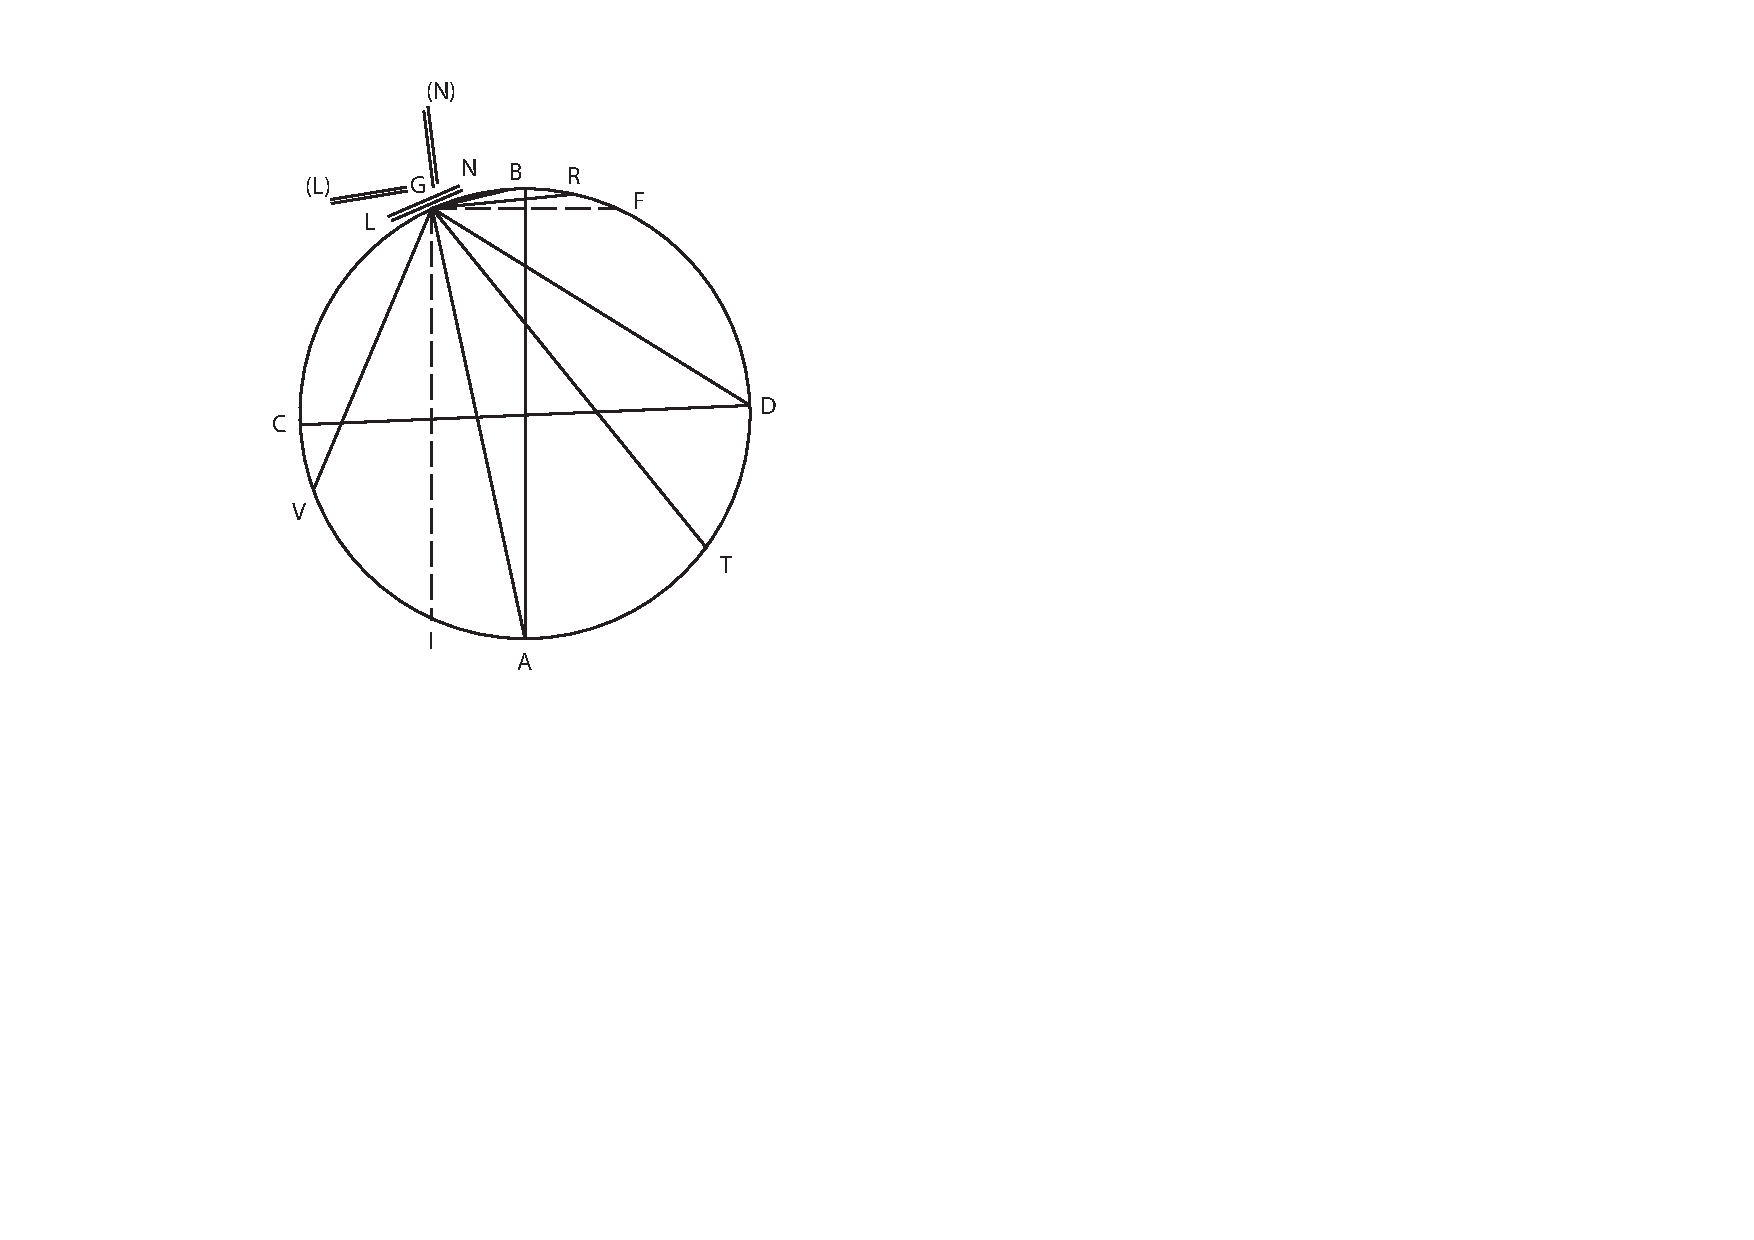
\includegraphics[trim = 0mm 2mm 0mm 0mm, clip,width=0.5\textwidth]{images/leotaud1668-d3.pdf}\\
\noindent \centering [\textit{Fig. 1}]
%\caption{Bildbeschreibung}
\end{center}
\vspace{0.15em}
\pstart%
[p. 99] [...] qua constat radios Aequatori\protect\index{Sachverzeichnis}{aequator} affines \edtext{ad distantiam non minorem Versoria ciere}{\lemma{}\Afootnote{\textit{Leibniz unterstreicht}: ad distantiam non minorem Versoria ciere.}}, quam Axi\protect\index{Sachverzeichnis}{axis} proximos [...]
\pend 
\pstart  [p. 188] [...] quodnam censebimus declinationum\protect\index{Sachverzeichnis}{declinatio} huiusmodi in eodem globo latere Principium? obseruabat \edtext{Cabeus\protect\index{Namensregister}{\textso{Cabeo}, Niccolò 1586-1650}}{\lemma{}\Afootnote{\textit{Leibniz streicht} Cabeus \textit{und schreibt}: Kircherus\protect\index{Namensregister}{\textso{Kircher}, Athanasius 1602-1680}.}}; et quidem, quod sciam [...]
\pend 
\pstart  [p. 190] Concedo itaque \edtext{Kirchero\protect\index{Namensregister}{\textso{Kircher}, Athanasius 1602-1680}}{\lemma{}\Afootnote{\textit{Leibniz unterstreicht}: Kirchero.}}, imo cum ipso contendo Magneticorum declinationes a Meridiano non aliunde ortum nancisci [...]
\pend 
\begin{center}                    
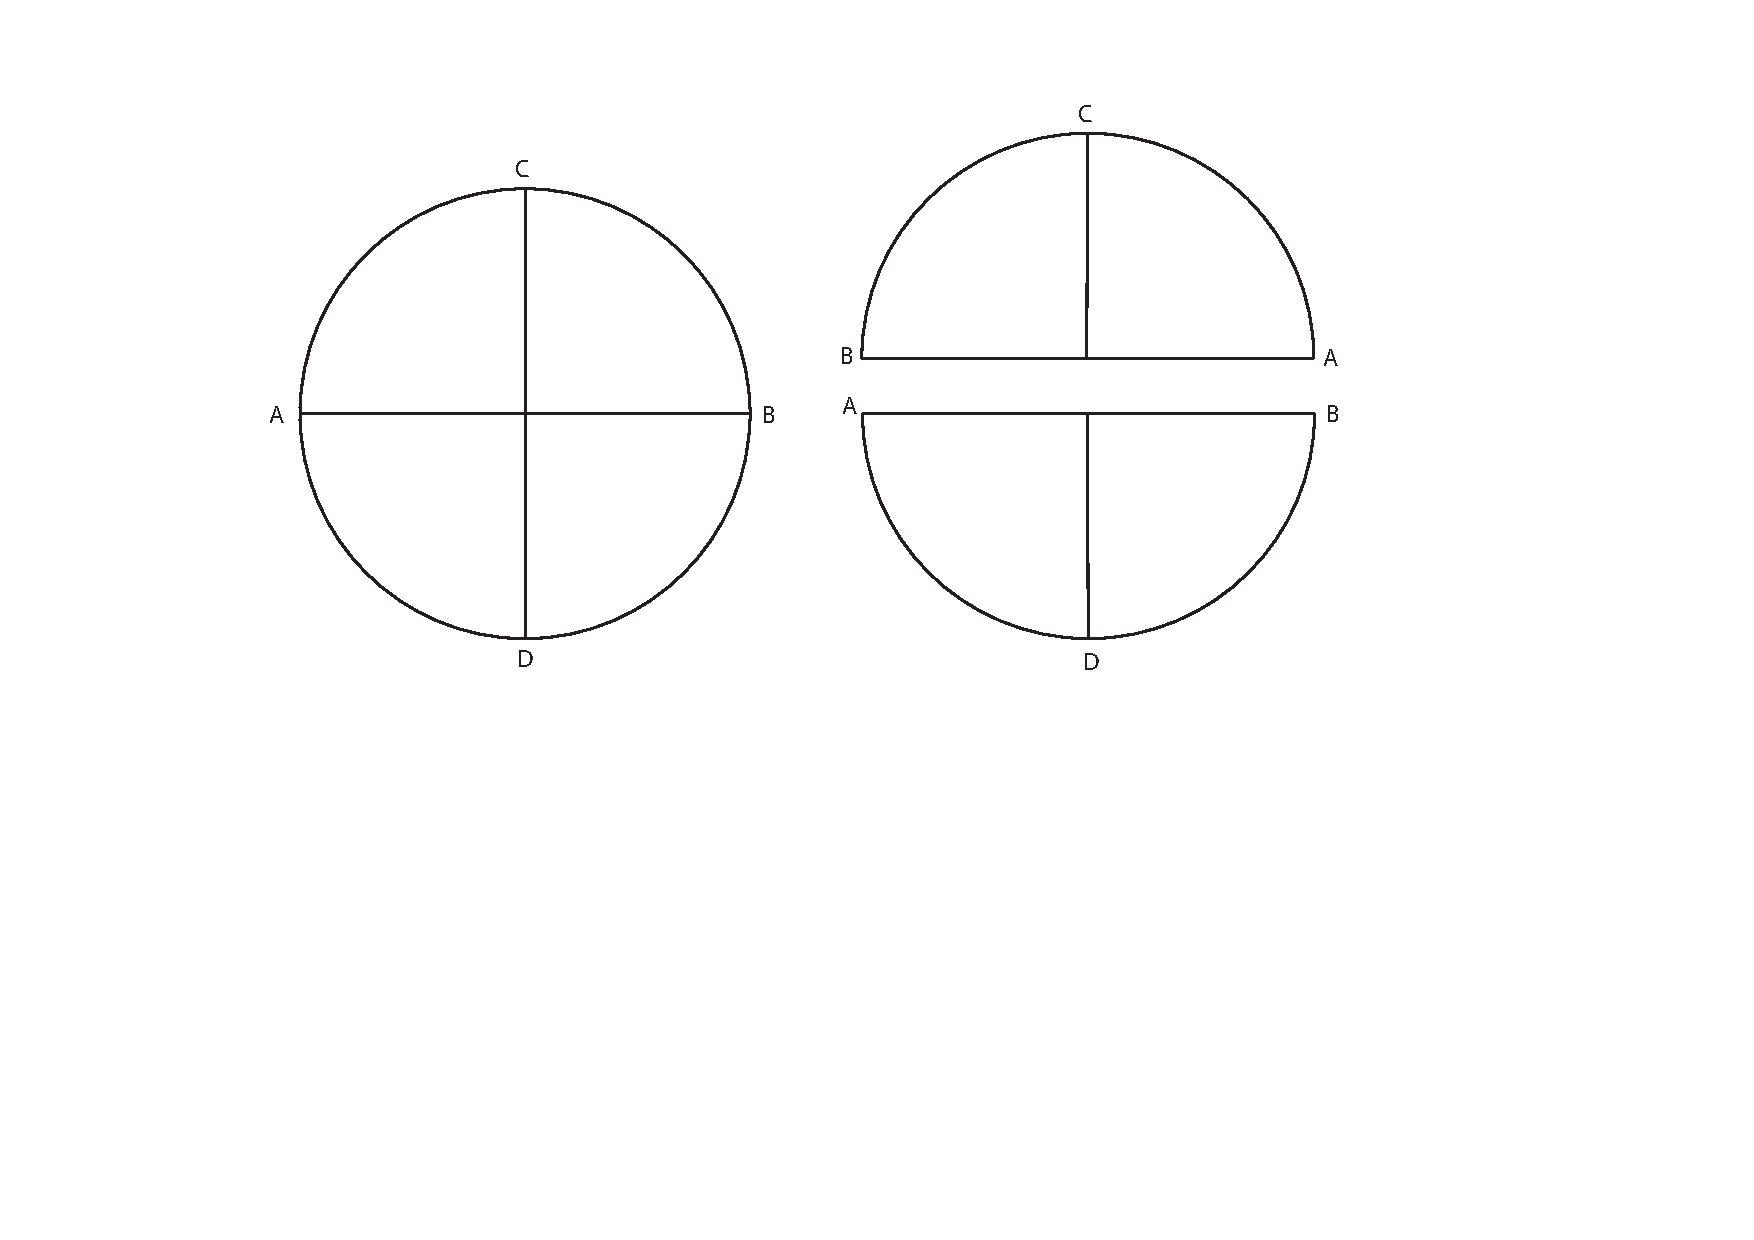
\includegraphics[width=1\textwidth]{images/leotaud1668-d4.pdf}\\
\noindent \centering [\textit{Fig. 2}] 
\end{center}
\vspace*{0.5em}
\pstart  [p. 191] Habes Principium\protect\index{Sachverzeichnis}{principium}, ex quo declinationes\protect\index{Sachverzeichnis}{declinatio} Magneticas oriri censet \edtext{Kircherus}{\lemma{}\Afootnote{\textit{Leibniz unterstreicht}: Kircherus\protect\index{Namensregister}{\textso{Kircher}, Athanasius 1602-1680}.}}, nempe Telluris partes insigniores rupibus, et scopulis interceptas [...]
\pend 
\pstart  [p. 254] Tantum abest, vt pars illa $A$ $C$ $B$ suspensa, et ad motum ineundum, quem vis imperabit Magnetica, expedita sese in ea positione ad partem alteram componat, quam ante diuisionem occupabat, cuique eam Natura ipsa nexu perpetuo ab ipso vsque Magnete\protect\index{Sachverzeichnis}{magnes} condito addixerat [...]
\pend
%\vspace{2em}
%\begin{center}                    
%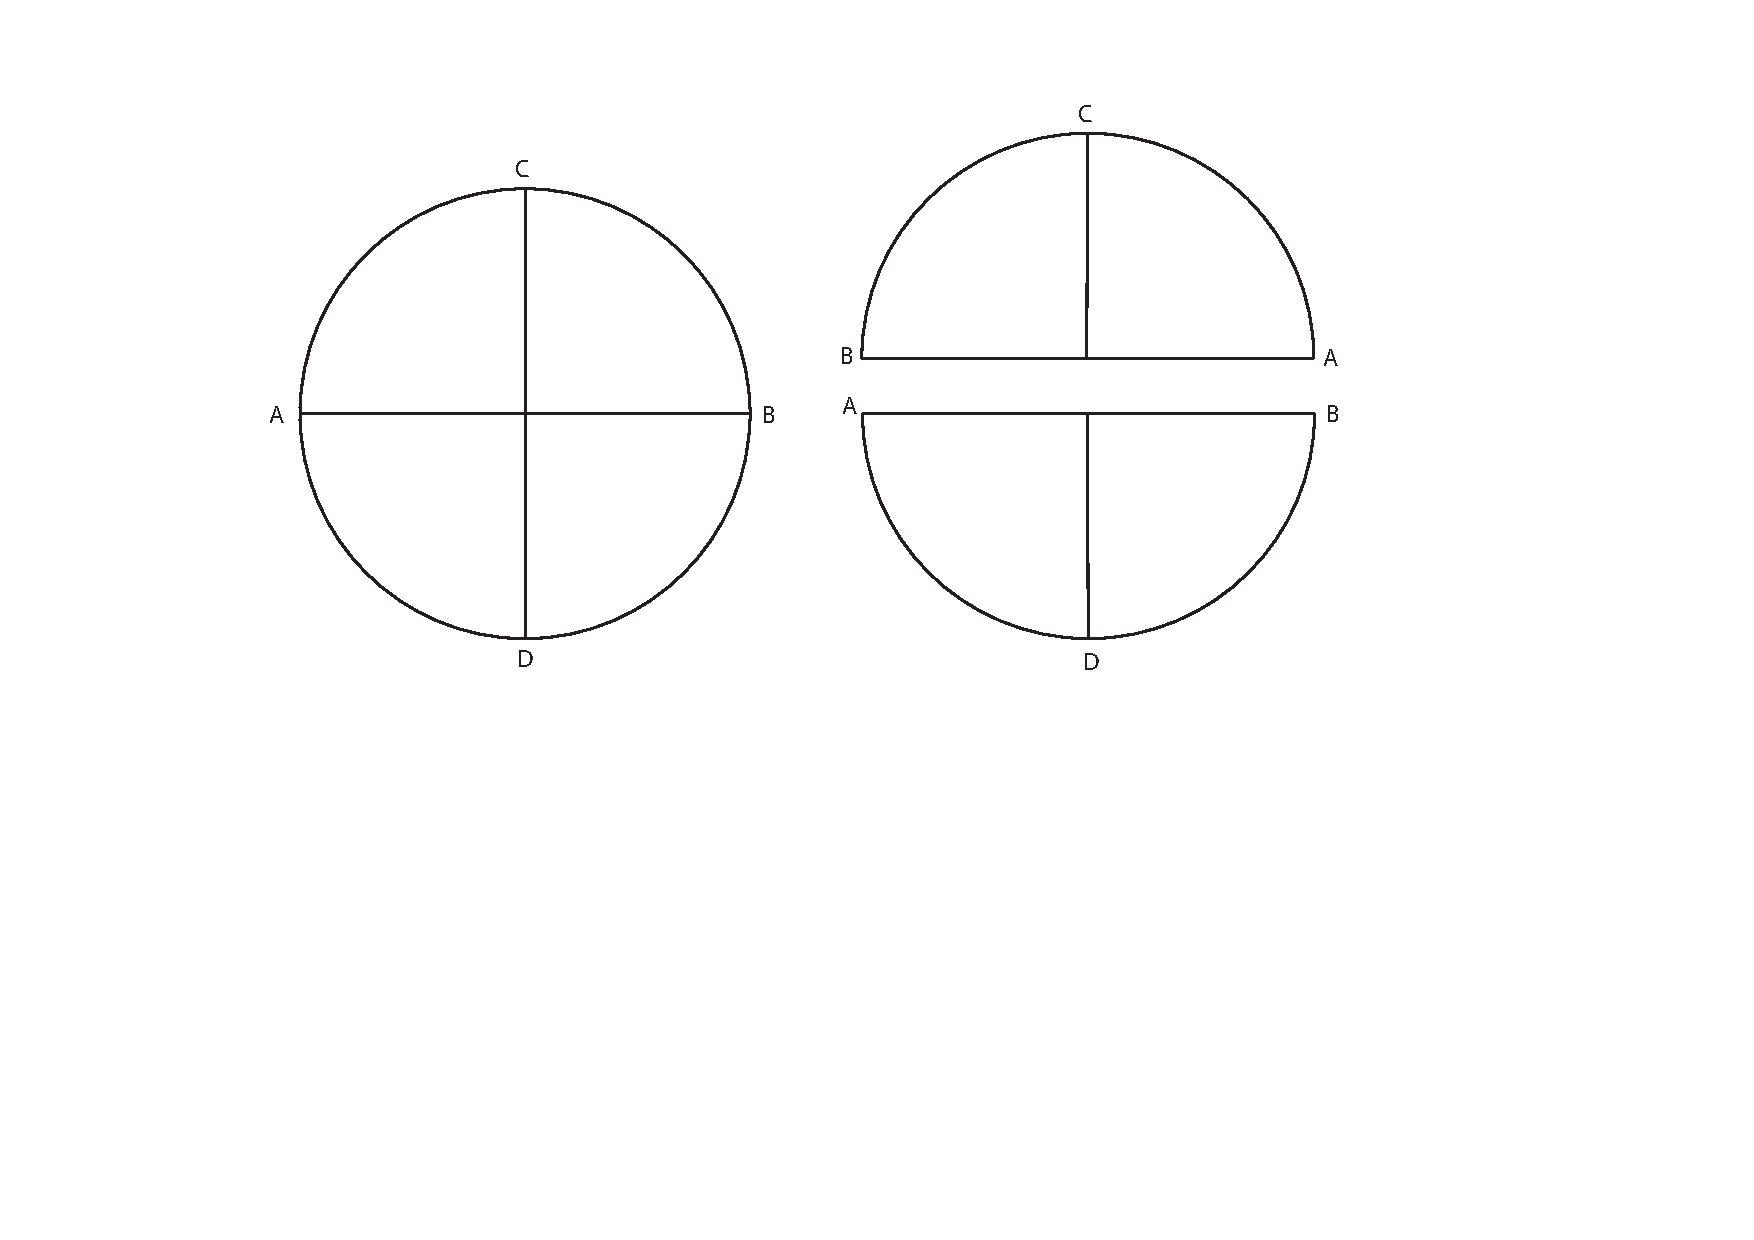
\includegraphics[width=1\textwidth]{images/leotaud1668-d4.pdf}\\
%\noindent \centering [\textit{Fig. 2}] \\
%\end{center}
\newpage
\pstart  
%\vspace*{-2mm}
[p. 256]
\pend
\count\Afootins=1000
\vspace*{-5mm}
\begin{center}                    
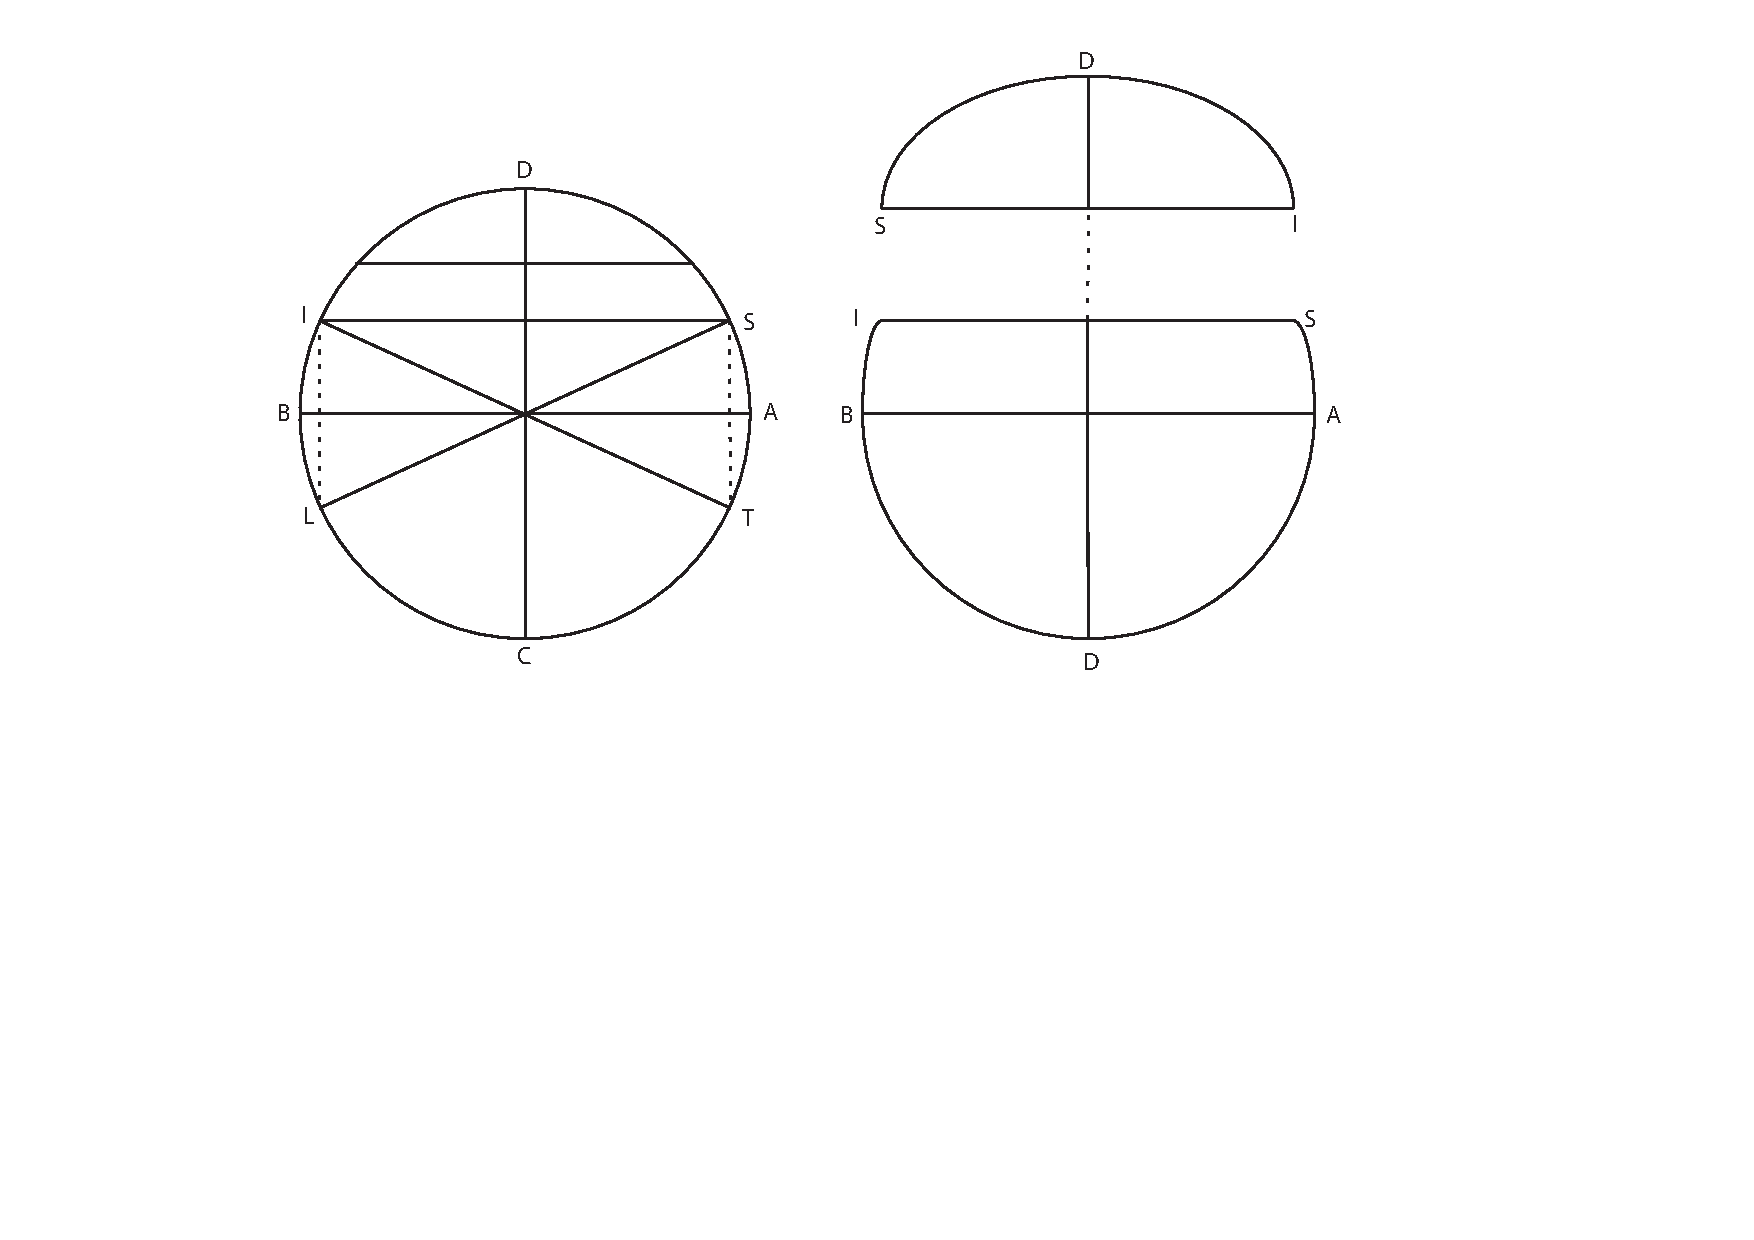
\includegraphics[width=0.96\textwidth]{images/leotaud1668-d1.pdf}\\
\noindent \centering [\textit{Fig. 3}] 
\end{center}
\pstart \edtext{}{\lemma{\hspace*{1.8mm}[\textit{Fig. 3}]}\killnumber\Afootnote{\textit{Leibniz streicht im linken Kreis den Durchmesser IT und im Kreissegment DIS die Sehne, deren Endpunkte nicht bezeichnet sind.}}}
Constat itaque ex iis, quae ibidem demonstrata sunt, obelum $IS$ firmiter eo in situ Magneti\protect\index{Sachverzeichnis}{magnes} incubare, nec sine vi aliqua ab ea abstrahi posse:
\pend 
\pstart [p. 257] Vt \textit{Lib.} 1. \textit{Cap.} 3. fusius declaratum est, Locum consule. Sed nunc ad rem nostram.
\pend
\pstart Cum itaque segmenti \textit{BCA} penduli [...]
\pend 
\count\Afootins=1200
\pstart
[p. 263] Cum enim partes illae Magnetis\protect\index{Sachverzeichnis}{magnes} diuisi suo loco restituuntur, agunt perinde, ac si continuae forent, omniaque puncta virtutis radios, vt prius emittunt, \edtext{nec in se mutuo agunt, sed simul coagunt}{\lemma{}\Afootnote{\textit{Leibniz unterstreicht}: nec in se mutuo agunt, sed simul coagunt.}} ad totalem effectum producendum [...]
\pend 
\pstart  [p. 296] \textso{ASSERTIO II.} /\edtext{\textit{Si ferrum, quamuis omni careat magnetica facultate, vni Magnetis Polo admoueatur: alter Magnetis\protect\index{Sachverzeichnis}{magnes} oppositus Polus ex ea ferri vnione robustior euadit.}}{\lemma{}\Afootnote{\textit{Leibniz markiert am Rand}: Si ferrum [...] robustior euadit.}} / Esto Magnes [...]
\pend 
\newpage
\begin{center}                    
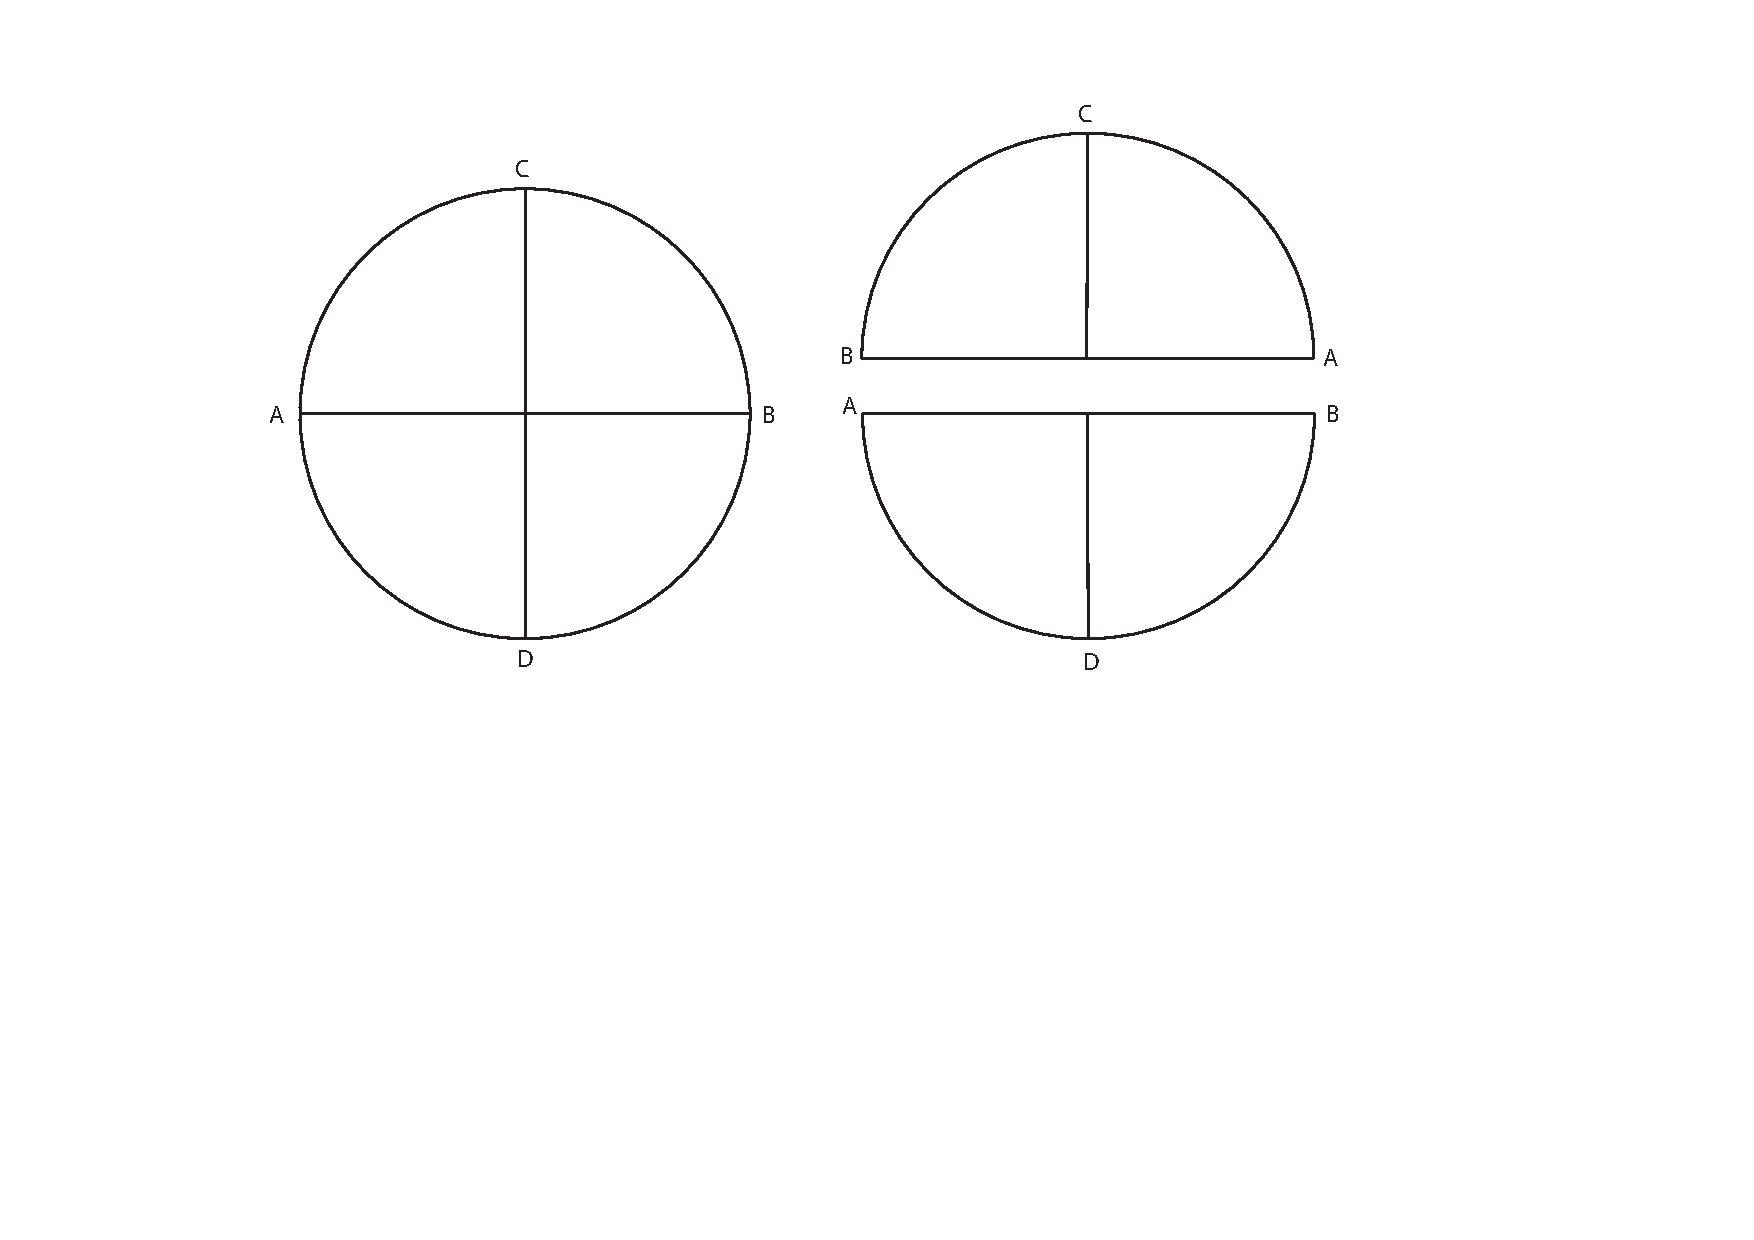
\includegraphics[width=1\textwidth]{images/leotaud1668-d2.pdf}\\
\noindent \centering [\textit{Fig. 4}] 
\end{center}
\vspace*{1em}
\pstart  [p. 298] \textso{ASSERTIO IV.} / \edtext{\textit{Quin etiam Magnes ad ferrum sibi adiungendum et suspendendum iuuatur ab alio ferro; licet hoc quam illud a Magnete\protect\index{Sachverzeichnis}{magnes} longius distet.}}{\lemma{}\Afootnote{\textit{Leibniz markiert am Rand die \"{U}berschrift}: Quin etiam [...] longius distet.}} \\In Schemate praecedente [...]
\pend 
%\newpage
\count\Afootins=1200
\pstart  [p. 315] Ratio huius effectus difficultatem non patitur, eaque expedita fuit superius \textit{Cap.} 2. in eo casu, \edtext{in quo scisso per Axem}{\lemma{}\Afootnote{\textit{Leibniz unterstreicht}: in quo scisso per Axem.}} aut Axi [p. 316] parallelam lineam Magnete\protect\index{Sachverzeichnis}{magnes} [...]
\pend 
\pstart  [p. 316] Ecce duo Magnetes $AB$ et $MS$, quorum duo poli poli $B$ et $S$ similes sunt, qui sese tangunt, aut a contactu non longe absunt, collatis ex aduerso infestis viribus ad vltimum vsque exitium decertant: \edtext{aut si sui iuris fuerint, et ad motum expediti, sine mora, qua licet, fugam capessunt, aut sese contorquent, ne aspectum quidem mutuum ferentes: tantis in se exardescunt odiis similes illae polorum $B$ et $S$ facies. Attamen amicissime conueniunt, sibique mutuam praestant operam, siue ad ferrum suspendendum, siue ad illud vehementiori facultate magnetica afficiendum.}{\lemma{}\Afootnote{\textit{Leibniz markiert am Rand}: sine mora [...] magnetica afficiendum.}} Sed haec nec noua sunt, nec insolita mysteria in Magneticis contemplationibus.
\pend 
\pstart  [p. 328] \edtext{Obseruatione porro dignum est duo huiusmodi Versoria lineam Meridianam nunquam occupare.}{\lemma{}\Afootnote{\hspace{3.5mm}\textit{Leibniz markiert am Rand}: Obseruatione porro [...] nunquam occupare.}} Etsi enim Telluris virtus ambas eorum cuspides versus plagam Septentrionalem adducat [...]
\pend 
\pstart
[p. 338] [...] dum enim $G$, vt eius virtus australis exigit, ad boream spectare molitur; \edtext{pari conatu oppositum $L$ ab australi polo vt infesto sese subducit, et ad borealem contendit. Quare tunc virgula illa non ante quietem adeptura est, quam medium inter boream et austrum situm sit assecuta; ita vt ad lineam meridianam perpendicularis statuatur vtrouis extremo $G$, aut $L$, provt fors tulerit}{\lemma{}\Afootnote{\textit{Leibniz markiert am Rand}: pari conatu [...] fors tulerit \textit{durch Strich und} NB.}}, ad ortum vel occasum converso; et quasi in aequilibrio stare compellatur pari vtrimque alliciente, pari arcente Telluris\protect\index{Sachverzeichnis}{tellus} virtute.
\pend 
\pstart  [p. 354] Nono. Si Magnetis\protect\index{Sachverzeichnis}{magnes} polus laminae ferreae in \edtext{rectanguli altera parte}{\lemma{}\Afootnote{\hspace{2.3mm}\textit{Leibniz unterstreicht}: rectanguli altera parte.}} longioris figuram efformatae ita applicetur, vt minoris lateris medium tangat: ea pene omnia euentura sunt, quae circa laminam circularem proxime sunt obseruata. \pend \pstart  [p. 355] Quare Si Magnetis polus $A$ lateri $GH$ adhaerens fuerit australis, australe etiam futurum est vtrumque latus $IG$, $LH$ (sunt enim hae duae facies, licet oblique, auersae, et exteriores ad faciem $A$ australem Magnetis\protect\index{Sachverzeichnis}{magnes}, adeoque eiusdem cum ipsa situs) facies vero $AE$ vtrique rectangulo $AI$, $AL$ communis, est borealis: \edtext{quia ad Magnetis faciem australem $A$, licet oblique, obuertitur, eique adhaeret, vt dissimilis et amica. Memoriam eorum refrica, quae de virgula ferrea $G$ $L$ Magnetis Polum\protect\index{Sachverzeichnis}{polus} $A$ tangente dicta sunt \textit{Num.} 2. idem enim hic contingere arguunt certa experimenta}{\lemma{}\Afootnote{\hspace{-1.9mm}\textit{Leibniz markiert am Rand}: quia ad Magnetis\protect\index{Sachverzeichnis}{magnes} [...] certa experimenta\protect\index{Sachverzeichnis}{experimentum}.}}: quae si deficerent, \edtext{vix ad id probandum rationes sufficerent}{\lemma{}\Afootnote{\hspace{2mm}\textit{Leibniz unterstreicht}: vix ad id probandum rationes sufficerent.}}; magnum enim prima fronte videtur discrimen intercedere inter virgulam illam, et hanc laminam [...]
\pend \pstart
[p. 357] Vnde tam repentina effectus huius mutatio? non nisi \edtext{ex duplici illo gladij ductu contrario}{\lemma{}\Afootnote{\hspace{1.2mm}\textit{Leibniz unterstreicht}: ex duplici illo gladij ductu contrario.}} supra eundem Magnetis polum.
\pend 
\newpage
\pstart
[p. 374] [...] vt non dubitem, quin Cabeus\protect\index{Namensregister}{\textso{Cabeo}, Niccolò 1586-1650} non sua doctus experientia\protect\index{Sachverzeichnis}{experientia}, sed Aliorum trita relatione deceptus contrarium asseruerit.
\pend 
\pstart
\edtext{Secundo vt certissima admitti debet capta a Gilberto\protect\index{Namensregister}{\textso{Gilbert}, William 1544-1603} experientia\protect\index{Sachverzeichnis}{experientia}, quam superius retuli. Nimirum, ferrum candens Versorio admotum nullo modo illud commouere; commouere autem statim vbi vehementior ille calor remittitur, etsi necdum totus euanuerit. Id saepius a me non sine admiratorum coetu tentatum, ab hoc euentu nunquam aberrauit. Suadeo, cum nihil facilius factu sit, vt periculum ipse facias; facies non sine voluptate, nec tantillae te poenitebit operae. Ex duobus hisce experimentis probatissimis a Kirchero, et Gilberto\protect\index{Namensregister}{\textso{Gilbert}, William 1544-1603} adductis, quae contrariam pene sententiam suadere videntur, nascitur grauissima difficultas, quae paulo post veniet excutienda: sed prius obseruandum est,}{\lemma{}\Afootnote{\textit{Leibniz markiert am Rand den Absatz}: Secundo vt [...] prius obseruandum est,}} 
\pend 
\pstart Tertio loco Rationem, quam Kircherus\protect\index{Namensregister}{\textso{Kircher}, Athanasius 1602-1680} affert, cur magnes ferrum candens prolectet, admitti non posse. 
\pend
\count\Afootins=1500
\count\Bfootins=1500
\count\Cfootins=1500

